% Copyright 2013 Mike Castleman, Meetup, Inc.
% This work is licensed under a Creative Commons Attribution 3.0
% United States License
% http://creativecommons.org/licenses/by/3.0/us/deed.en_US
\documentclass{beamer}
\mode<presentation>
{
  \usecolortheme{seagull}
  \usetheme{Madrid}
}
\usepackage[english]{babel}
\usepackage{fontspec}
\usepackage{xunicode}
\usepackage{xltxtra}
\usepackage{url}
\usepackage{polyglossia}
\usepackage{xcolor}
\usepackage{listings}

\setsansfont[Mapping=tex-text,ItalicFont={* Italic}]{Roboto}
\setmonofont{Droid Sans Mono}
\setdefaultlanguage{english}

\definecolor{mauve}{rgb}{0.58,0,0.82}
\definecolor{dkgreen}{rgb}{0.2,0.9,0.2}
\lstset{%
  language=XML,
  basicstyle=\scriptsize\tt,
  breaklines=true,
  showspaces=false,
  showstringspaces=false,
  keywordstyle=\color{blue},
  commentstyle=\color{dkgreen}\addfontfeature{FakeBold=1.5},
  stringstyle=\color{mauve},
  numberstyle=\color{red!75}
}

\title[Android Resources]{Resources on Android}

\author{Mike Castleman}
\institute{Meetup}
\date[DevFest 2013]{ADI DevFest, 2013-02-04}

\pgfdeclareimage[height=0.5cm]{meetup-logo}{meetup-logo}
\logo{\pgfuseimage{meetup-logo}}

\begin{document}

\begin{frame}
  \titlepage
\end{frame}

\begin{frame}{Fragmentation}
\Large{``Developing for Android is hard, because there are lots of different
devices, and you have to test your app on every single one of them.''
\vskip 3em
--- People who never develop for Android}
\end{frame}

\begin{frame}{Resources}
\begin{itemize}
\item Provide different assets for different devices
\item Let the platform choose the right one
\item Set things up \textit{declaritively}: don't write any extra code!
\end{itemize}
\end{frame}

\begin{frame}{Resource Types}
\begin{itemize}
\item \texttt{drawable}: images etc.
\item \texttt{layout}
\item \texttt{values}: strings, styles, themes, integers, arrays
\item \texttt{anim}, \texttt{color}, \texttt{menu}
\item \texttt{xml}, \texttt{raw}
\end{itemize}
\end{frame}

\begin{frame}{Qualifiers}
\begin{itemize}
\item OS Version: \texttt{v9} etc.
\item Screen size: \texttt{small}, \texttt{medium} (phones);
  \texttt{large}, \texttt{xlarge} (tablets)
\item Language (and country): \texttt{en}, \texttt{es},
  \texttt{en-rCA}
\item Portrait/landscape: \texttt{port}, \texttt{land}
\item Screen density: \texttt{ldpi}, \texttt{mdpi}, \texttt{hdpi}, \texttt{xhdpi}
\item Many others, see SDK docs if interested.
\end{itemize}
\end{frame}

\begin{frame}{Directory structure}
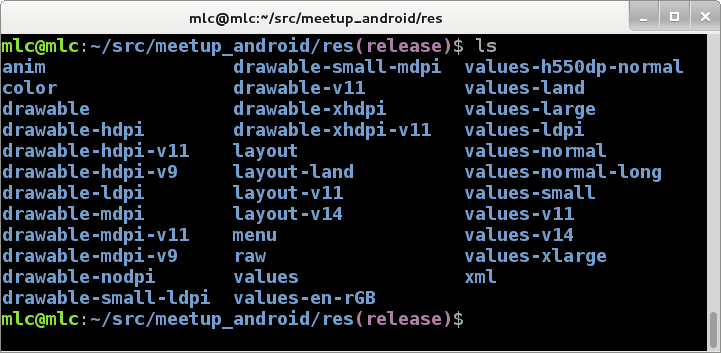
\includegraphics[width=3.5in]{dir.png}
\end{frame}

\begin{frame}{Use cases}
\begin{tabular}{cc}
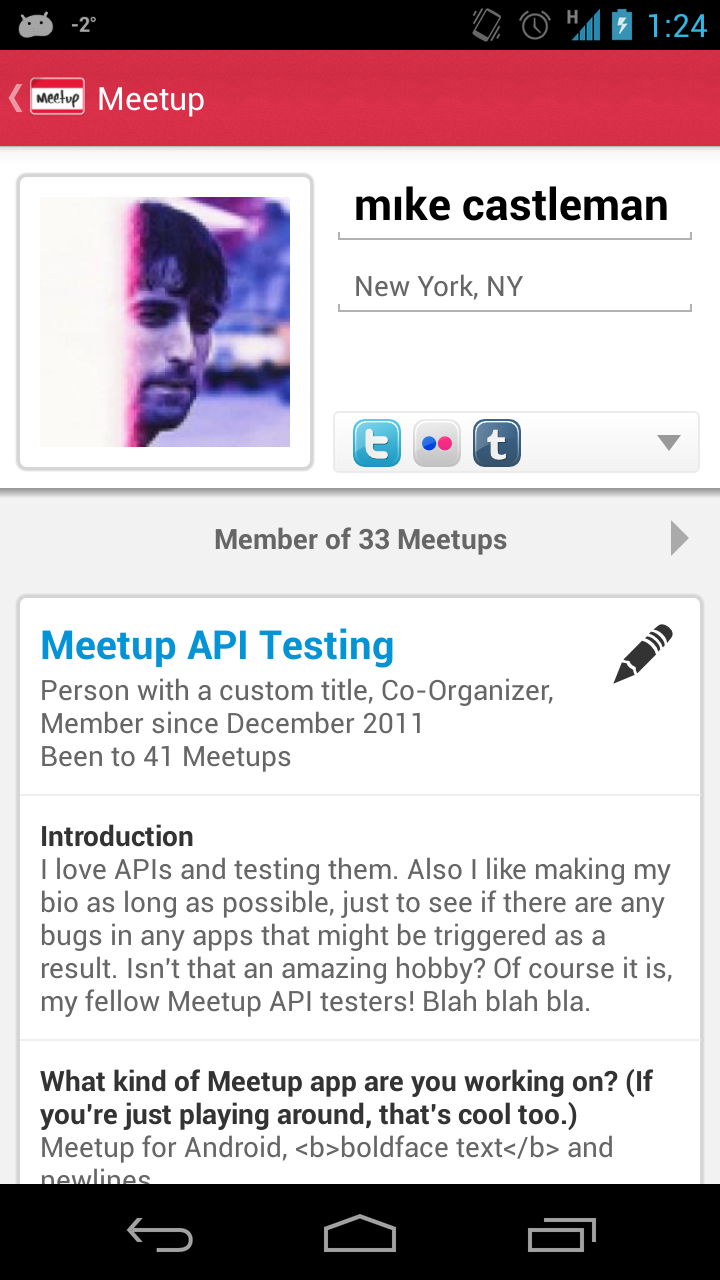
\includegraphics[width=1.5in]{layout.png} &
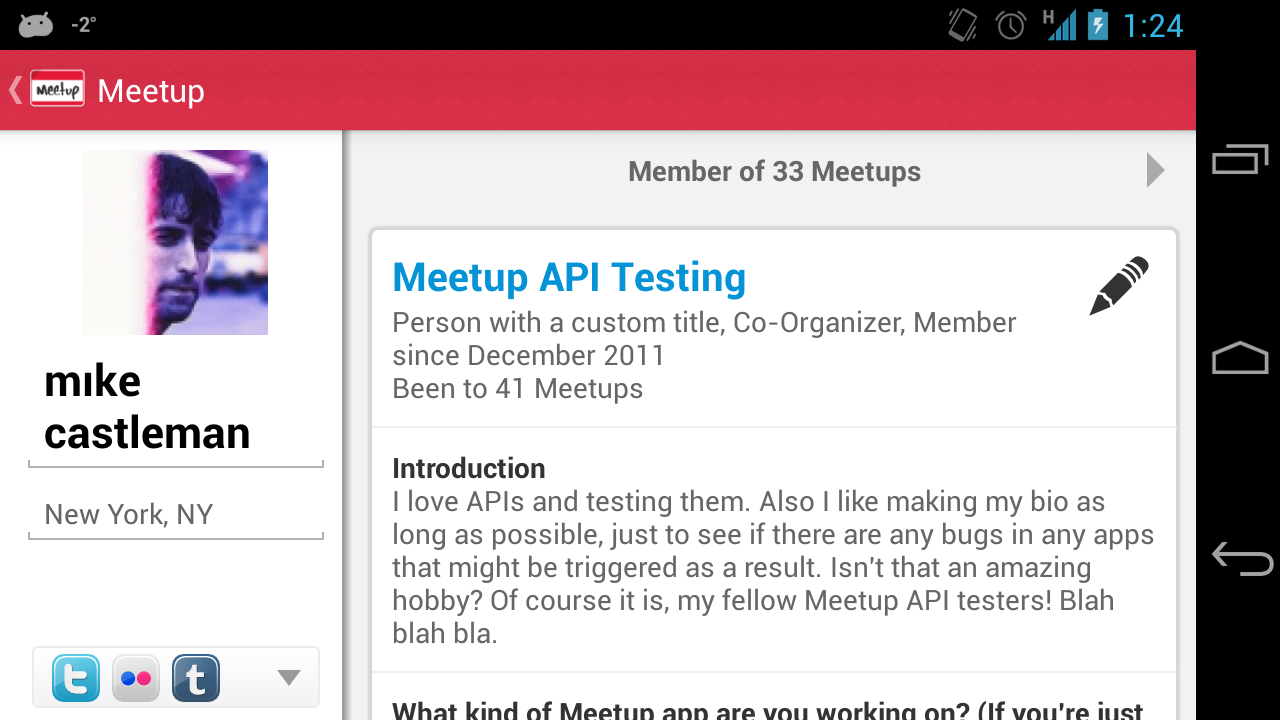
\includegraphics[height=1.5in]{layout-land.png} \\
\texttt{res/layout} & \texttt{res/layout-land}
\end{tabular}
\end{frame}

\begin{frame}{Use cases}
\centerline{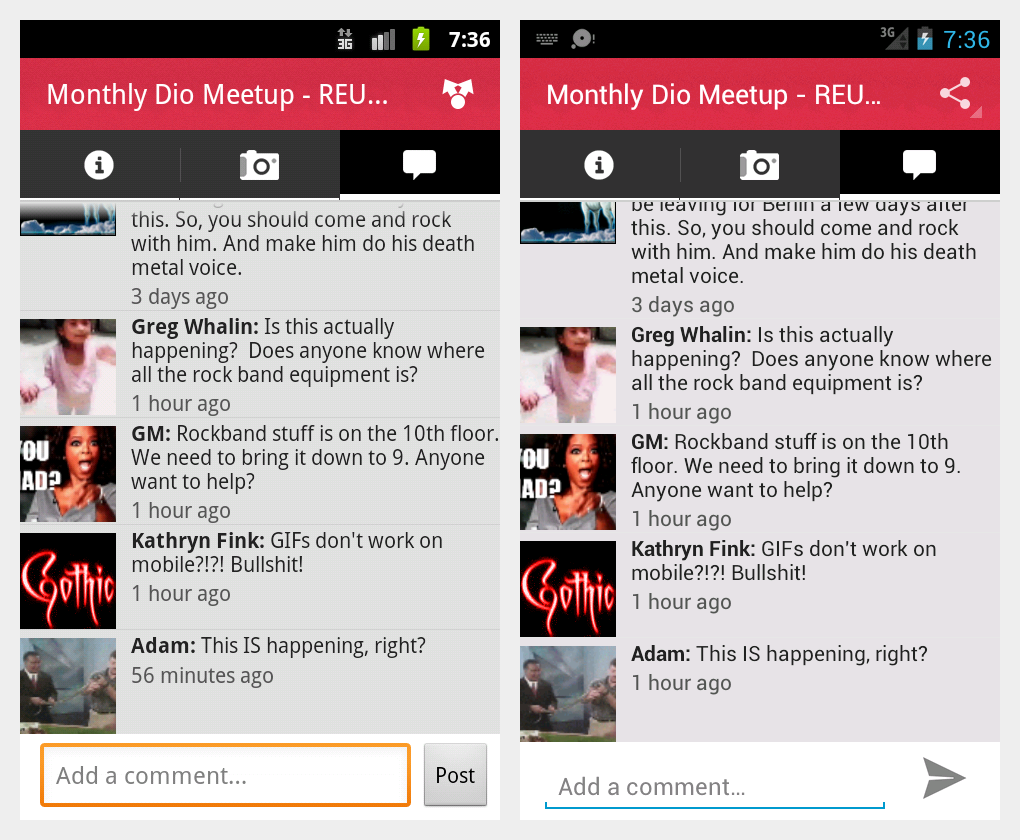
\includegraphics[width=3.25in]{api-levels.png}}

\centerline{\texttt{res/values/styles.xml}\ \ \texttt{res/values-v11/styles.xml}}
\end{frame}

\begin{frame}[fragile]{Use cases}
\begin{itemize}
\item \texttt{res/values/strings.xml}
\begin{lstlisting}
<string name="nice_phone">Nice phone!</string>
<string name="nice_tablet">Nice tablet!</string>
<string name="nice_device">@string/nice_phone</string>
\end{lstlisting}
\item \texttt{res/values-large/strings.xml}
\begin{lstlisting}
<string name="nice_device">@string/nice_tablet</string>
\end{lstlisting}
\item \texttt{res/values-it/strings.xml}
\begin{lstlisting}
<string name="nice_phone">Bel telefono!</string>
<string name="nice_tablet">Bel tablet!</string>
\end{lstlisting}
\item \texttt{res/layout/activity.xml}
\begin{lstlisting}
<TextView android:id="@+id/praise_user_device"
    android:layout_width="match_parent"
    android:layout_height="wrap_content"
    android:text="@string/nice_device"/>
\end{lstlisting}
\end{itemize}
\end{frame}

\begin{frame}[fragile]{Nononono}
\begin{lstlisting}[language=Java]
public class TurnBlueOnTouch implements View.OnTouchListener {
  @Override
  public boolean onTouch(View v, MotionEvent event) {
    if (event.getActionMasked() == MotionEvent.ACTION_DOWN)
      v.setColor(Color.argb(255, 0, 0, 127));
    else if (event.getActionMasked() == MotionEvent.ACTION_UP)
      v.setColor(Color.BLACK);
    return false;
  }
}
\end{lstlisting}
\end{frame}

\begin{frame}[fragile]{Yesyesyesyes}
\begin{lstlisting}
<selector xmlns:android="http://schemas.android.com/apk/res/android">
  <item android:state_pressed="true" android:color="#ff00007f" />
  <item android:color="@color/black" />
</selector>
\end{lstlisting}
\end{frame}

\begin{frame}{Images: Four ``Abstract Densities''}
\begin{itemize}
\item \texttt{ldpi}: 75\% of base
\item \texttt{mdpi}: base image size
\item \texttt{hdpi}: 150\% of base
\item \texttt{xhdpi}: 200\% of base
\end{itemize}
\begin{tabular}{cccc}

\includegraphics[scale=0.5]{jogdial_l.png} &

\includegraphics[scale=0.5]{jogdial_m.png} &

\includegraphics[scale=0.5]{jogdial_h.png} &

\includegraphics[scale=0.5]{jogdial_xh.png} \\
\texttt{ldpi} & \texttt{mdpi} & \texttt{hdpi} & \texttt{xhdpi} \\
48×48 & 64×64 & 96×96 & 128×128
\end{tabular}
\end{frame}

\begin{frame}{Images: Measurement Units}
\begin{itemize}
\item \texttt{px} --- physical device pixels
\item \texttt{dp} --- ``density-independent pixel''
\end{itemize}
On \texttt{mdpi}, 1 px = 1 dp. Not so on other densities!

Devices vary both in their density and in their size in dp.
\end{frame}

\begin{frame}{But!}
\begin{itemize}
\item Android will automatically scale if you don't have appropriate
  files.
\item \texttt{ldpi} maybe irrelevant.\\
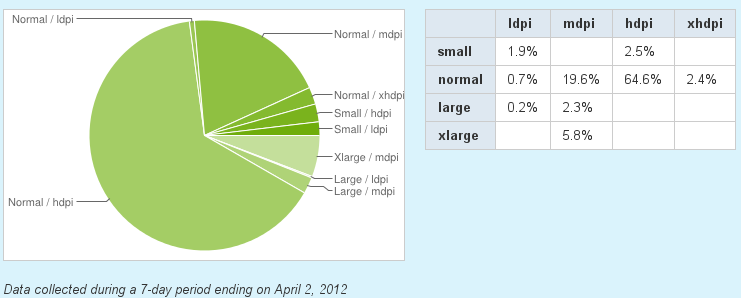
\includegraphics[width=3.5in]{densities.png}
\item Maybe just \texttt{xhdpi} if you're feeling brave.
\end{itemize}
\end{frame}

\begin{frame}{9-Patch Images}
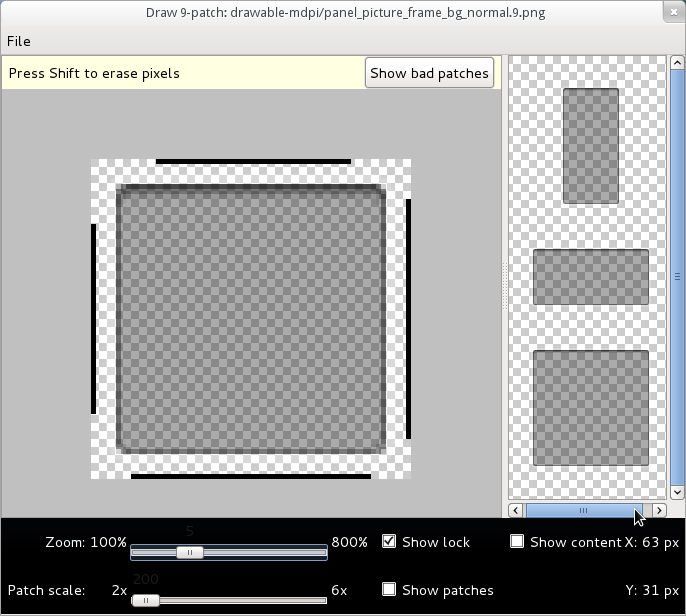
\includegraphics[width=3.25in]{draw9patch.png}
\end{frame}

\begin{frame}{Thank You}
Questions?

\vskip 2em
Also, we're hiring, interns and full-time positions:\\
\texttt{jobs@meetup.com}
\end{frame}
\end{document}


